\documentclass[border=6pt]{standalone}
\usepackage{amsmath,amssymb}
\usepackage{tikz}
\usetikzlibrary{arrows.meta,calc,decorations.pathreplacing,patterns,shapes.geometric,positioning,shadings}

\begin{document}
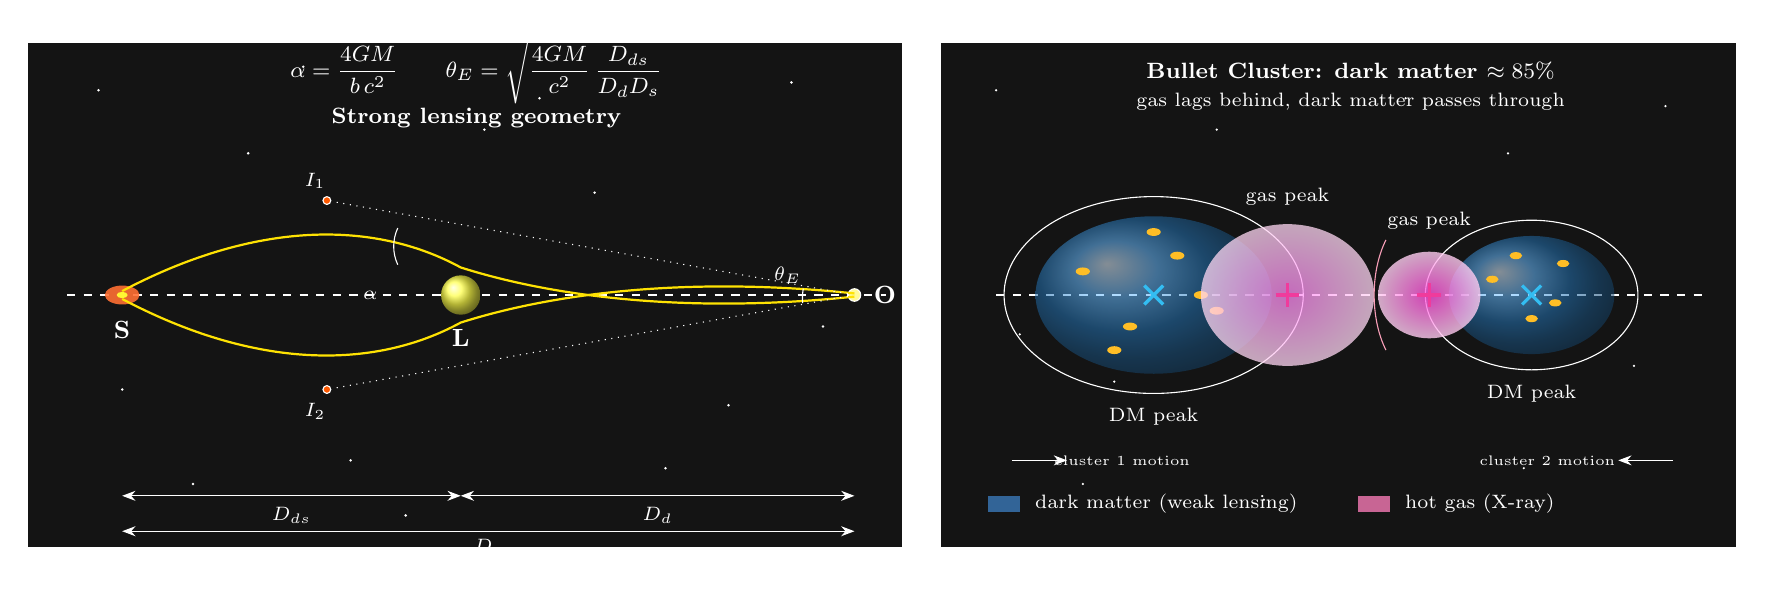
\begin{tikzpicture}[>=Stealth]

% ===========================================================
% LEFT PANEL: Gravitational Lensing Geometry
% ===========================================================
\begin{scope}[local bounding box=left]

% Dark night-sky background
\fill[black!92] (-0.3,-3.2) rectangle (10.8,3.2);

% faint background stars
\foreach \x/\y in {0.6/2.6, 1.8/-2.4, 3.2/2.9, 4.5/-2.8, 6.2/2.5, 7.8/-2.2, 9.4/2.7, 2.5/1.8, 8.6/-1.4, 0.9/-1.2, 5.5/2.1, 6.9/1.3, 3.8/-2.1, 9.8/-0.4}{
  \fill[white!80] (\x,\y) circle (0.5pt);
}

% Optical axis
\draw[white!45, dashed, thin] (0.2,0) -- (10.6,0);

% Observer O (right side)
\node[circle, fill=yellow!40, draw=white, inner sep=1.6pt] (O) at (10.2,0) {};
\node[white, font=\small\bfseries, right=1pt of O] {O};

% Lens L (middle) -- mass, pale yellow
\shade[ball color=yellow!70] (5.2,0) circle (0.25);
\node[circle, inner sep=0pt] (L) at (5.2,0) {};
\node[white, font=\small\bfseries] at (5.2,-0.55) {L};

% Source S (left side) -- small ellipse galaxy
\begin{scope}[shift={(0.9,0)}]
  \fill[orange!60!red!80, opacity=0.9] (0,0) ellipse (0.22 and 0.12);
  \fill[yellow!80] (0,0) ellipse (0.07 and 0.04);
\end{scope}
\node[white, font=\small\bfseries] at (0.9,-0.45) {S};

% Two light rays (gold), symmetric, bent toward L
% upper ray: S -> just above L -> O
\draw[yellow!85!orange, thick]
  (0.9,0.05) .. controls (2.6,0.95) and (4.1,0.95) .. (5.2,0.35)
             .. controls (6.3,0.0) and (8.0,-0.25) .. (10.2,-0.02);
% lower ray: S -> just below L -> O
\draw[yellow!85!orange, thick]
  (0.9,-0.05) .. controls (2.6,-0.95) and (4.1,-0.95) .. (5.2,-0.35)
              .. controls (6.3,0.0) and (8.0,0.25) .. (10.2,0.02);

% Images I1 (upper) and I2 (lower) -- where observer thinks source is
% Observer sees image along tangent of incoming ray direction
\node[circle, fill=orange!70!red, draw=white, inner sep=1pt] (I1) at (3.5,1.2) {};
\node[circle, fill=orange!70!red, draw=white, inner sep=1pt] (I2) at (3.5,-1.2) {};
\node[white, font=\scriptsize] at (3.35,1.45) {$I_1$};
\node[white, font=\scriptsize] at (3.35,-1.48) {$I_2$};

% Apparent-image sight lines from O (dotted)
\draw[white!55, dotted] (O) -- (I1);
\draw[white!55, dotted] (O) -- (I2);

% Deflection angle alpha at L (upper ray)
\draw[white!75, thin] (4.4,0.85) arc[start angle=155, end angle=205, radius=0.55];
\node[white, font=\scriptsize] at (4.05,0.0) {$\alpha$};

% Einstein angle theta_E at O
\draw[white!75, thin] (9.55,0.08) arc[start angle=170, end angle=185, radius=0.7];
\node[white, font=\scriptsize] at (9.35,0.25) {$\theta_E$};

% Distance labels D_d, D_ds, D_s
% D_d: O to L (below)
\draw[white!70, <->, thin] (5.2,-2.55) -- (10.2,-2.55);
\node[white, font=\scriptsize] at (7.7,-2.8) {$D_d$};

% D_ds: L to S (below)
\draw[white!70, <->, thin] (0.9,-2.55) -- (5.2,-2.55);
\node[white, font=\scriptsize] at (3.05,-2.8) {$D_{ds}$};

% D_s: O to S (lower, full span)
\draw[white!60, <->, thin] (0.9,-3.0) -- (10.2,-3.0);
\node[white, font=\scriptsize] at (5.55,-3.2) {$D_s$};

% Formulas (top of left panel)
\node[white, font=\footnotesize] at (5.4,2.85)
  {$\alpha=\dfrac{4GM}{b\,c^{2}}\qquad
    \theta_E=\sqrt{\dfrac{4GM}{c^{2}}\,\dfrac{D_{ds}}{D_d D_s}}$};

\node[white, font=\footnotesize\bfseries] at (5.4,2.25) {Strong lensing geometry};

\end{scope}

% ===========================================================
% RIGHT PANEL: Bullet Cluster schematic
% ===========================================================
\begin{scope}[xshift=11.6cm, local bounding box=right]

% Dark background
\fill[black!92] (-0.3,-3.2) rectangle (9.8,3.2);

% faint background stars/galaxies
\foreach \x/\y in {0.4/2.6, 1.5/-2.4, 2.7/2.8, 3.8/-2.6, 5.6/2.5, 7.1/-2.2, 8.9/2.4, 1.9/-1.1, 6.9/1.8, 8.5/-0.9, 3.2/2.1, 0.7/-0.5}{
  \fill[white!75] (\x,\y) circle (0.45pt);
}

% Horizontal reference line for the four peaks
\draw[white!25, dashed, thin] (0.4,0) -- (9.4,0);

% --- Two galaxy-cluster outlines (white thin, not filled) ---
% Left cluster outline (bigger)
\draw[white, thin] (2.4,0) ellipse (1.9 and 1.25);
% Right cluster outline (smaller, the "bullet")
\draw[white, thin] (7.2,0) ellipse (1.35 and 0.95);

% --- Dark matter halos (cool blue), centered on the cluster positions ---
\shade[ball color=cyan!55!blue!80, opacity=0.55]
  (2.4,0) ellipse (1.5 and 1.0);
\shade[ball color=cyan!55!blue!80, opacity=0.55]
  (7.2,0) ellipse (1.05 and 0.75);

% Small galaxies scattered inside each cluster (yellow-orange tiny ellipses)
\foreach \x/\y in {1.5/0.3, 2.1/-0.4, 2.7/0.5, 3.2/-0.2, 2.4/0.8, 3.0/0.0, 1.9/-0.7}{
  \fill[orange!60!yellow!85] (\x,\y) ellipse (0.09 and 0.05);
}
\foreach \x/\y in {6.7/0.2, 7.2/-0.3, 7.6/0.4, 7.0/0.5, 7.5/-0.1}{
  \fill[orange!60!yellow!85] (\x,\y) ellipse (0.08 and 0.045);
}

% --- Hot X-ray gas clouds (pink), lagging BETWEEN the two clusters ---
% Main gas cloud shifted right of left cluster (lagging behind)
\shade[inner color=magenta!70!pink!60, outer color=magenta!35!pink!30, opacity=0.75]
  (4.1,0) ellipse (1.1 and 0.9);
% Bow-shock "bullet" gas (just left of right cluster center)
\shade[inner color=magenta!80!red!70, outer color=magenta!40!pink!35, opacity=0.80]
  (5.9,0) ellipse (0.65 and 0.55);

% bow-shock arc in front of bullet
\draw[magenta!30!pink!80, thin]
  (5.35,0.7) .. controls (5.15,0.3) and (5.15,-0.3) .. (5.35,-0.7);

% --- Four peak markers on the horizontal line ---
% Dark matter peaks (blue crosses)
\draw[cyan!80, very thick] (2.4,0) ++(-0.12,-0.12) -- ++(0.24,0.24);
\draw[cyan!80, very thick] (2.4,0) ++(-0.12,0.12) -- ++(0.24,-0.24);
\draw[cyan!80, very thick] (7.2,0) ++(-0.12,-0.12) -- ++(0.24,0.24);
\draw[cyan!80, very thick] (7.2,0) ++(-0.12,0.12) -- ++(0.24,-0.24);

% Gas peaks (pink plus)
\draw[magenta!70!pink, very thick] (4.1,0) ++(-0.15,0) -- ++(0.3,0);
\draw[magenta!70!pink, very thick] (4.1,0) ++(0,-0.15) -- ++(0,0.3);
\draw[magenta!70!pink, very thick] (5.9,0) ++(-0.15,0) -- ++(0.3,0);
\draw[magenta!70!pink, very thick] (5.9,0) ++(0,-0.15) -- ++(0,0.3);

% Peak labels
\node[white, font=\scriptsize] at (2.4,-1.55) {DM peak};
\node[white, font=\scriptsize] at (7.2,-1.25) {DM peak};
\node[white, font=\scriptsize] at (4.1,1.25) {gas peak};
\node[white, font=\scriptsize] at (5.9,0.95) {gas peak};

% Direction arrows showing collision motion
\draw[white!80, ->, thin] (0.6,-2.1) -- (1.3,-2.1);
\node[white, font=\tiny] at (2.0,-2.1) {cluster 1 motion};
\draw[white!80, <-, thin] (8.3,-2.1) -- (9.0,-2.1);
\node[white, font=\tiny] at (7.4,-2.1) {cluster 2 motion};

% Caption / legend
\node[white, font=\footnotesize\bfseries] at (4.9,2.85)
  {Bullet Cluster: dark matter $\approx 85\%$};
\node[white, font=\scriptsize] at (4.9,2.45)
  {gas lags behind, dark matter passes through};

% Legend swatches
\fill[cyan!55!blue!80, opacity=0.7] (0.3,-2.75) rectangle (0.7,-2.55);
\node[white, font=\scriptsize, right=2pt] at (0.7,-2.65) {dark matter (weak lensing)};
\fill[magenta!60!pink!75, opacity=0.8] (5.0,-2.75) rectangle (5.4,-2.55);
\node[white, font=\scriptsize, right=2pt] at (5.4,-2.65) {hot gas (X-ray)};

\end{scope}

\end{tikzpicture}
\end{document}
